\chapter{Desenvolvimento do controlador}
\label{ch:desenvolvimento_controlador}

Com o intuito de controlar o \acrshort{tclabsp} aplicando o \acrshort{mpc} como técnica,
utilizaram-se os modelos teóricos e experimentais apresentados nas \cref{sec:modelagem_da_planta_piloto}
e \cref{sec:modelo_experimental} para o desenvolvimento do bloco controlador no \textit{Simulink}.
Um controlador \acrshort{pid} também foi desenvolvido a fim de servir como base comparativa ao
controlador \acrshort{mpc} criado.
A seção a seguir descreve este controlador \acrshort{pid}

% =====================================================================================================
% ============================================= Section ===============================================
% =====================================================================================================
\section{Controlador PID}
\label{sec:controlador_pid}

O controlador \acrshort{pid} desenvolvido e descrido nesta seção foi criado em ambiente \textit{Simulink},
utilizando o aplicativo \textit{PID Tuner} do \acrshort{matlab}, disponível através do pacote
\textit{Control System Toolbox}.

A cada um dos Aquecedores do \acrshort{tclabsp} foi conectado a um bloco \textit{PID Controller} retroalimentado
com a saída dos Sensores de Temperatura da planta, conforme ilustrado pela \cref{fig:pidcreation}.

\begin{figure}[h]
	\caption{Modelo Simulink do controlador PID}
	\begin{center}
		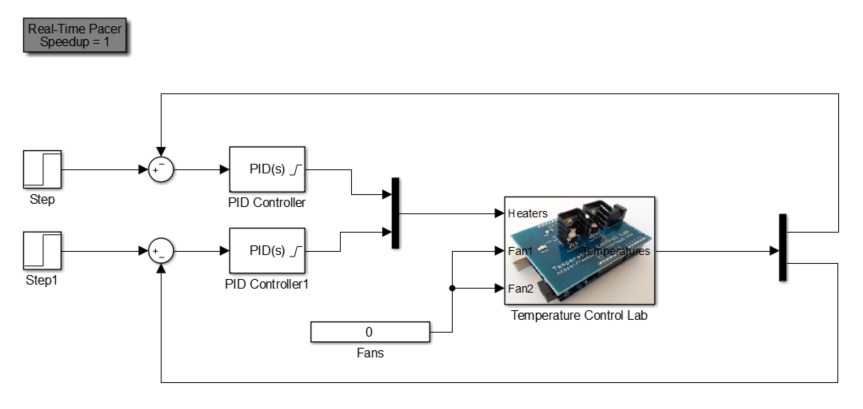
\includegraphics[width=1.00\textwidth]{./5_images/PIDCreation.png} 
		\label{fig:pidcreation}
	\end{center}
	\centering
	\makebox[\width]{Fonte: Autor} 
\end{figure}

Os blocos \textit{PID Controller} foram inicialmente configurados com os limites de saturação de saída
entre 0 e 100 para que nenhum valor fora desta faixa fosse aplicado a planta controlada.
Em seguida, uma vez que o desenvolvimento do controlador \acrshort{pid} não era um objetivo deste trabalho,
utilizou-se a função de auto-sintonia do \textit{PID Tuner} para encontrar valores satisfatórios de controle
do sistema.

A \cref{tab:pid_values} apresenta os valores de sintonia encontrados para um controlador \acrshort{pid}
paralelo (\cref{eq:pid_format}).

\begin{equation}
    \label{eq:pid_format}
    P + I \frac{1}{s} + D \frac{N}{1 + N \frac{1}{s}}
\end{equation}

\begin{table}[h]
	\centering
	\caption{Sintonia dos blocos PID}
	\label{tab:pid_values}
	\begin{tabular}{c|cc} \toprule
		{Parâmetro}		            & {PID Aquecedor 1}     & {PID Aquecedor 2}           \\ \midrule
		Proporcional (P)		    & $1.435$               & $2.182$                     \\
		Integral (I)   		        & $0.016$               & $0.011$                     \\
		Derivativo (D)		        & $-9.119$              & $-30.919$                   \\
		Filtro (N)                  & $0.0216$              & $0.010$                     \\ \bottomrule
	\end{tabular}
	\caption*{Fonte: Autor}
\end{table}


% =====================================================================================================
% ============================================= Section ===============================================
% =====================================================================================================
\section{Controlador MPC}
\label{sec:controlador_mpc}